\documentclass[11pt, a4paper]{article}
\usepackage[english, serbian]{babel}

\usepackage{float}
\usepackage{xcolor}
\usepackage{graphicx}
\usepackage{adjustbox}
\usepackage{caption}
\usepackage{authblk}
\usepackage{geometry}
\usepackage{adjustbox}
\usepackage{amssymb, amsmath, bm}
\usepackage{textcomp}
\usepackage{booktabs}
\usepackage[textfont=it, tableposition=top]{caption}
\usepackage[%
colorlinks=true,
pdfborder={0 0 0},
linkcolor=red
]{hyperref}
\geometry{
	a4paper,
	total={166mm,253mm},
	left=22mm,
	top=22mm,
}

\captionsetup[table]{name=Tabela}
\captionsetup[figure]{name=Figura}

\definecolor{cc-blue}{HTML}{1f77b4}
\definecolor{cc-orange}{HTML}{ff7f0e}
\definecolor{cc-green}{HTML}{2ca02c}
\definecolor{cc-red}{HTML}{d62728}
\definecolor{cc-purple}{HTML}{9467bd}

\title{Revizori sistema za prepoznavanje lica -- etička pitanja\\\small{Seminarski rad u okviru kursa\\računarstvo i društvo\\Matematički fakultet}}
\author{Kosta Grujčić\\mi17012@alas.matf.bg.ac.rs}

\begin{document}
\maketitle

\begin{abstract}
    Iako ključni u otkrivanju pristrasnosti, dobronamerni pokušaji algoritamskog revizionisanja mogu imati kontraefekat upravo po populaciju koju nameravaju da zaštite. Ova zabrinutost posebno dolazi do izražaja prilikom provere biometrijskih sistema poput prepoznavanja lica, gde su podaci vrlo osetljivi, a tehnologija obično ne prati sve etičke standarde. Kroz pet \textit{etičkih pitanja} u domenu verifikacije tehnologije prepoznavanja lica, podeljenih na preglede dizajna i etičke konfilkte biće analizirano algoritamsko revizionisanje opisivanjem uloge i principa rada.
\end{abstract}

\tableofcontents

\section{Uvod}
Tehnologija analize lica (eng. \textit{FPT}) je opšti pojam koji obuhvata razne probleme poput detekcije lica (pronalaženje lica na slici), ispitivanja lica (utvrđuje demografske ili fizičke karakteristike pojedinca) i identifikacije lica (utvrđuje identitet pojedinca).

FPT ima širok dijapazon primene poput merenja zadovoljstva mušterija detekcijom osmeha, utvrđivanja demografskih karakteristika određene populacije, do praćenja pojedinaca \cite{G37}. Korporativna retorika uspešne primene ovakvih sistema se koristi izjavama poput \textit{razumevanje korisnika}, \textit{praćenje i detekcija ljudskih aktivnosti}, \textit{pretraživanje biblioteka digitalnih slika}, \textit{identifikovanje subjekata u bezbednosnim situacijama} \cite{G1, G8, G16, G33}.

FPT sistemi su zapravo vrlo ranjivi, pogotovo u primeni nadzora u sprezi sa gramzivim prikupljanjem podataka, kada, bilo to namerno ili nenamerno, diskriminišu manjinske grupe \cite{G2}. Rizik je veći time što kompanije poput Amazon-a ili HireVue-a naplaćuju svoje usluge policijskim upravama ili koriste pomenute tehnologije prilikom zapošljavanja kandidata \cite{G5, G43}.

Mnoge organizacije za zaštitu prava građana su izrazile zabrinutost za sisteme prepoznavanja lica i skrenule pažnju ka kreiranju politike kontrole i regulacije primene. Nekoliko država u Sjedinjenim Američkim Državama poput Kalifornije, Vašingtona, Teksasa, Ilinoja, Ajdaha, kao i nekoliko gradova poput San Franciska, Ouklenda i Somervila, su vodeći kada je reč o kontroli ili potpunoj zabrani pomenutih sistema. Do januara 2020. godine predloženo je nekoliko zakonskih regulativa u SAD (\textit{Algorithmic Accountability Act} \cite{G9}, \textit{Commercial Facial Recognition Privacy Act of 2019} \cite{G4} and No Biometric Barriers Act \cite{G10}), dok je u Velikoj Britaniji nacrtom predložen moratorijum \cite{G11}.

Neki od ovih predloga u svojim memorandumima eksplicitno savetuju da se rezultati FPT revizora kao što je \textit{Gender Shade} \cite{G6} i drugih standarda razvijenih od strane Nacionalnog Instituta za Standarde i Tehnologiju koriste kao preduslov za akreditaciju, odnosno moratorijum, FPT sistema. Ovi predlozi formulišu revizore kao pouzdan mehanizam za potvrdu bezbedne i proverene upotrebe.

%Doprinosi ovog istraživanja su sledeći. Razvili smo novi skup podataka CelebSET, koji će služiti kao referenca za ovakav vid testiranja i sastoji se od slika poznatih ličnosti. Na ovom skupu podataka ćemo testirati trenutno komercijalno dostupne FTP API-eve. Zatim ćeno izvršiti analizu po principu studije slučaja i izneti sve relevantne etičke aspekte algoritamskog revizionisanja.

\section{CelebSET: etalon za FPT}
Skupovi podataka kao što su FRVT, IARPA, IJB \cite{G38}, PPB \cite{G6} su se pokazali kao ključni za otkrivanje pristrasnosti u problemima detekcije lica, verifikacije, identifikacije, klasterovanja identitata i prepoznavanja pola. Revizije sprovedene nad ovim skupovima podataka su uticale na mnoga skorija istraživanja na temu nedostatka raznovrsnosti u FPT testovima. Predložen je frejmvork za evaluaciju pristrasnosti u domenu klasifikacije u isporučenim sistemima \cite{G32, G43, G45}. Pređašnja istraživanja su proveravala isključivo komercijalne modele po pitanju rodne/polne i rasne diskriminacije u FPT. Iako postoji izvestan broj referentnih testova za evaluaciju većeg broja klasifikacionih problema u FPT, ali niti jedan ne dopušta takvo testiranje na višem nivou apstrakcije (eng. \textit{black box}). \\
\indent U cilju prevazilaženja tog problema, kreiran je novi referentni skup podataka -- CelebSET. Predstavlja podskup IMDB-WIKI skupa podataka \cite{G40} i sadrži 80 identita poznatih ličnosti i to po 20 za svaku od naredne četiri grupe: tamni muškarci (DM), tamne žene (DF), svetli muškarci (LM) i svetle žene (LF). Informacije o rasnoj pripadnosti poznatih ličnosti su preuzeti sa sajta famousfix.com i ethnicelebs.com, a potom upareni sa IMDB-WIKI skupom podataka. Grupa D je dobijena uzimanjem slika osoba označenih kao crnci uz vizuelnu inspekciju konsultovanjem Flicpatrikove skale boje kože \cite{G41} (u rasponu od 3 do 6). Grupa L je dobijena analogno. Metapodaci za grupe F i M su dobijeni direktno iz IMDB-WIKI skupa podataka. Uzrast osobe je izračunat kao razlika datuma nastanka fotografije i datuma rođenja. Za svaku osobu je odabrano po 10 slika na kojima se smeje, odnosno ne smeje. \\
\indent Korišćene su izvorne slike sa označenim okvirima dobijenih iz IMDB-WIKI skupa podataka \cite{G40} za potrebe revizije na problemu detekcije. Korišćene su isečene slike sa licima iz originalnog skupa podataka za potrebe revizije na problemu analize lica.

\subsection{Provera API-eva na CelebSET-u}
Izvršićemo proveru API-eva objavljenih od strane Microsoft-a, Amazon-a i Clarifai-a, koji imaju najveći opseg delanja. Microsoft je značajan i zbog ispitivanja u okviru \textit{Gender Shades} istraživanja \cite{G6}, dok je Amazon-ov API proveren u okviru nastavka pomenutog istraživanja, \textit{Actionable Auditing} \cite{G39}. Međutim, Clarifai nije obrađen ni u jednom istraživanju koji se tiče revizionisanja. Za probleme poput automatskog prepoznavanja pola, detekcije lica i identifikacije imena, tačnost se izražava kao odstupanje od ciljnih veličina. Za problem predviđanja uzrasta, dozvoljava se odstupanje od 8 godina radi prilagođavanja izlazu Amazon-ovog API-a. Uspešnost detekcije se kvantifikuje koristeći $AP_{50}$ (eng. \textit{average precision}) metriku.

\begin{table}[h!]
	\centering
	\caption{\textbf{Sveukupne performanse na odabranim problemima predviđanja karakteristika lica.}}
	\begin{tabular}{c|ccccc} \toprule
		{} & {Pol} & {Uzrast} & {Ime} & {Osmeh} & {Detekcija} \\ \midrule
		{Microsft} & 99.94\% & 74.09\% & 98.69\% & 79.94\% & 93.56\% \\ 
		{Amazon} & 99.75\% & 58.40\% & 87.25\% & 94.16\% & 99.25\% \\
		{Clarifai} & 85.97\% & 55.24\% & 95.00\% & 56.19\% & 99.31\%\\ \bottomrule
	\end{tabular}
	\label{table:overall}
\end{table}

\begin{table}[h!]
	\centering
	\caption{\textbf{Razlika uspešnosti na subjektima svetlije (L) i tamnije (D) boje kože.}}
	\begin{tabular}{c|ccccc} \toprule
		{} & {Pol} & {Uzrast} & {Ime} & {Osmeh} & {Detekcija} \\ \midrule
		{Microsft} & 0.13\% & 18.35\% & 1.41\% & -0.48\% & 3.38\% \\ 
		{Amazon} & 0.25\% & 16.83\% & 1.03\% & -0.75\% & 0.25\% \\
		{Clarifai} & 11.69\% & 1.00\% & 7.50\% & 0.12\% & 0.42\%\\ \bottomrule
	\end{tabular}
	\label{table:unitary-color}
\end{table}

\begin{table}[h!]
	\centering
	\caption{\textbf{Razlika uspešnosti na subjektima muškog (M) i ženskog (F) pola.}}
	\begin{tabular}{c|ccccc} \toprule
		{} & {Pol} & {Uzrast} & {Ime} & {Osmeh} & {Detekcija} \\ \midrule
		{Microsft} & 0.13\% & 9.90\% & 1.23\% & -4.45\% & 0.62\% \\ 
		{Amazon} & 0.00\% & 12.28\% & 4.75\% & -9.00\% & 0.50\% \\
		{Clarifai} & 7.58\% & 10.26\% & -1.01\% & 1.25\% & -1.63\%\\ \bottomrule
	\end{tabular}
	\label{table:unitary-gender}
\end{table}

\begin{table}[h!]
	\centering
	\caption{\textbf{Razlika uspešnosti između najboljih i najgorih intersekcionalnih podgrupa za svaki od problema. Podgrupe su tamnopute žene (DF), tamnoputi muškarci (DM) i belci za oba pola (LF i LM). Podebljane vrednosti ukazuju na istovetnu uspešnost. Konkretno, 0.25\% (DM/LM/LF-DF) znači da je razlika uspešnosti između DM i DF, LM i DF, LF i DF jednaka i iznosti 0.25\%.}}
	\begin{adjustbox}{width=\textwidth}
	\begin{tabular}{c|ccccc} \toprule
		{} & {Pol} & {Uzrast} & {Ime} & {Osmeh} & {Detekcija} \\ \midrule
		{Microsft} & 0.25\% (\textbf{DM/LM/LF-DF}) & 29.47\% (LF-DF) & 3.90\% (LF-DF) & 8.02\% (LF-LM) & 4.25\% (LM-DM) \\ 
		{Amazon} & 0.50\% (LF-DF) & 29.10\% (LM-DF) & 6.71\% (DM-DF) & 9.75\% (DF-LM) & 0.75\% (\textbf{LM-DF/LF}) \\
		{Clarifai} & 19.10\% (LM-DF) & 11.21\% (LM-DF) & 10.50\% (LM-DF) & 3.00\% (LF-LM) & 0.50\% (\textbf{LM/LF-DF}) \\ \bottomrule
	\end{tabular}
	\end{adjustbox}
	\label{table:intersectional}
\end{table}


\begin{table}[h!]
	\centering
	\caption{\textbf{Udeo etničkih grupa prema komercijalno dostupnim API-evima.}}
	\begin{adjustbox}{width=\textwidth}
	\begin{tabular}{c|cccccccc} \toprule
		{} & {Azijati} & {Belci} & {Hispano} & {Crnci} & {Arapi} & {Indijci} & {Ostalo} & {Ukupno} \\ \midrule
		{Microsft API} & 7,838 & 15,536 & 10 & 8,816 & 995 & 1,316 & 7,167 & 41,678 \\
		{} & 18.8\% & 37.3\% & 0.02\% & 21.1\% & 2.4\% & 3.2\% & 17.2\% & 100.0\% \\ \midrule
		{Clarifai API} & 172 & 4,861 & 0 & 534 & 31 & 125 & 800 & 6,523 \\
		{} & 2.6\% & 74.5\% & 0.0\% & 8.2\% & 0.5\% & 1.9\% & 12.3\% & 100.0\% \\ \bottomrule
	\end{tabular}
	\end{adjustbox}
	\label{table:ethnicity-api}
\end{table}

\subsubsection{Sveukupne performanse} Kao što se vidi u tabeli \ref{table:overall}, svi API-evi postižu najbolje rezultate na problemu klasifikacije pola, sa izuzetkom Clarifai-a koji je najbolji na detekciji lica. Važno je reći da su Amazon-ova i Microsoft-ova rešenja već podvrgnuta proveri na problemu klasifikacije polova, nakon čega su objavljene ažurirane verzije \cite{G6, G39}. Sva rešenja pokazuju najgore rezultate na problemu predviđanja uzrasta.

\subsubsection{Performanse na unitarnim podgrupama} Tabele \ref{table:unitary-color} i \ref{table:unitary-gender} pokazuju da, uz izvesne izuzetke, svi API-evi imaju najlošije rezultate na subjektima tamnije boje kože kao i osobama ženskog pola, što je već poznato iz \cite{G6}. Clarifai, jedini komercijalan API koji do sad nije podvrgnut testiranju, pokazuje značajno veće odstupanje na svim unitarnim podgrupama za razliku od konkurenata.

\subsubsection{Performanse na intersekcionalnim podgrupama} Tabela \ref{table:intersectional} prikazuje uspešnost na intersekcionalnim podgrupama i potvrđuje već pomenuti zaključak -- podgrupa na kojoj se sva rešenja pokazuju lošije je podgrupa tamnoputih žena, dok podgrupa belih muškaraca ima najbolje rezultate.

\section{Detaljan pregled etičkog pitanja}
Koristeći reviziju sa CelebSET-om kao primer, podrobno će biti objašnjeno etičko pitanje algoritamskog revizionisanja. Uočavaju se \textit{pregledi dizajna} i \textit{etički konfilkti} kao dve grupe grube podele etičkog pitanja. Pregledi dizajna se bave detaljima na koje treba obratiti pažnju tokom revizije u cilju što bolje ocene testiranog sistema. S druge strane, etički problemi se odnose na situacije u kojima se dve ili više etički ispravnih odluka nađu u konfliktu.

\subsection{Pregledi dizajna}
\subsubsection{Pregled 1: Definisanje opsega delovanja}
Algoritamsko revizionisanje može pogoditi određenu demografsku grupu, konkretan problem ili kompaniju. Ovako uzak opseg ciljeva omogućava efikasnije uklanjanje visoko rizičnih pretnji i propusta. S druge strane, jednako smanjuje opseg delovanja revizija i dozvoljava preprilagođavanje na konkretnim problemima. \\
\indent U praksi, pouzdanost rezultata revizije zavisi i od relevantnosti podataka korišćenih u procesu revizije. Relevantnost ima prostornu i vremensku dimenziju. Ukoliko nije definisano kada se određeni referentni skup podataka treba koristiti, tada ne možemo znati ni kada rezultat revizije više nije od značaja. Analogno, nema smisla vršiti reviziju u cilju provere određene demografske grupe nad nekim skupom podataka ukoliko taj skup zapostavlja istu tu grupu. \\
\indent\textbf{Ilustracija} Revizije vršene nad CelebSET-om ukazuju da na ovakve vrste eksternih revizija treba gledati kao na mehanizme odgovornosti u sklopu vrlo uskog domena primene. Na primer, Clarifai ima diskrepancu od 19.10\% između najbolje i najgore demografske grupe na problemu određivanja pola, ponavaljajući rezultat iz izvornog \textit{Gender shade} istraživanja \cite{G6} i pokazujući daleko lošije rezultate u odnosu na konkurenciju (Microsoft i Amazon). Zapravo, Microsoft i Amazon imaju najmanja odstupanja na problemu određivanja pola, upravo na problemu nad kojim su prethodne revizije i vršene. Podsećanja radi, nakon tih revizija su obe kompanije predstavile ažurirane API-eve. To potvrđuje rezultate iz \textit{Actionable Auditing} istraživanja -- prethodno revizionisani API-evi imaju bolje rezultate na CelebSET-u što doprinosi perzistenciji pristranosti \cite{G39}.\\
\indent Interesantno, ne samo da to važi za kompanije čiji se proizvodi testiraju, već se istovetno dešava i problemima koji se testiraju. U okviru CelebSET revizije, API-evi od Amazon-a i Microsoft-a se najgore pokazuju na problemu određivanja uzrasta. Slično se primećuje i za ostale probleme. To može značiti da eksterna algoritamska revizija podstiče kompanije da otklone nedostatke svojih rešenja koja su podvrgnuta testiranju. \\
\indent Kompanije isto tako nastoje da poboljšaju rezultate na podgrupama koje su bile predmet prethodnih istraživanja (npr. binarni polovi ili vrsta kože). Budući da je većina revizionisanih API-eva namenjena sprovođenju zakona u SAD \cite{G7}, imigracionim i vojnim službama \cite{G18, G30}, stavljanje akcenta na učinak prema vrsti kože može imati smisla u slučaju procene rizika kod ljudi čija je boja kože često dovoljan razlog dodatnih provera. Međutim, postoje i druge manjinske grupe kao i slučajevi koji se mogu prevideti. Na primer, problem u radu algoritma za analizu lica je zaključao naloge transrodnim Uber vozačima \cite{G31}. Ove i slične situacije su dale povod rešavanju problema izraženih dispariteta određenih demografskih grupa \cite{G42}. \\
\indent Iako je važno postići jednak učinak na svim podgrupama na nekom od problema, revizori to ne smeju da zahtevaju ukoliko je to pogubno po određene zajednice. Problem klasifikacije pola nad kojim su kompanije minimizovale grešku, ima štetan efekat u slučaju i dobre i loše klasifikacije. Konkretno, može dovesti do podsticanja polnih stereotipa \cite{G19}, do potpunog isključenja transrodnih i ne-binarnih pojedinaca kao i rodno neusaglašenih pojedinaca, pa i do ugrožavanja već marginalizovanih grupa \cite{G22}. Prema tome, smanjivanje odstupanja tačnosti nije nužno etički podobno.

\subsubsection{Pregled 2: Revizija zarad pravičnosti postupka}
Nije dovoljno samo razmatrati metrike revizije. Da bi se FPT sistem adekvatno testirao, reviziju je potrebno shvatiti ozbiljnije od pukog poređenja brojeva na nekom referentnom skupu. U cilju povećanja naplate poreza korist ima primena pristupa proceduralne pravičnosti tokom procesa revizije. Primera radi, istraživanja u Australiji i Maleziji nastoje da odgovore kompanije od traženja rupa u zakonu, među kojima se najviše ističe utaja poreza. Umesto klasičnog pregledanja dokumenata koje bi druga strana predala, revizori utvrđuju u kojoj su meri kompanije izmirivale svoje obaveze \cite{G17, G36} tako što procenjuju komplijansu proveravanjem interne dokumentacije. Rezultat ovakvog vida revizije je daleko revnosnije izmirivanje obaveza. Slični zaključci se mogu videti u drugim istraživanjima poput \cite{G14, G15}. \\
\indent U nekim slučajevima se u domenu mašinskog učenja, pravičnost postupka ogleda u metodima interpretacije koji pokušavaju da oktriju kako se određeni izlaz dostiže. Kada je reč o problemima automatizovane analice lica, utvrđuje se koji delovi slike najviše utiču na krajnji rezultat, pritom vodeći računa da osetljive informacije poput rase ne smeju biti uzete u obzir. Kako je određeno rešenje konstruisano, vrste testova koji su vršeni, dostupna dokumentacija i uputstva su vrlo važni atributi takve analize. FPT evaluacije poput \textit{Face Recognition Vendor Test} (FRVT) Nacionalnog instituta za standarde i tehnologiju, sadrže neki stepen ovih razmatranja, poput sveobuhvatnog testa upotrebe rešenja \cite{G38}. Potreba za kompletnim revizorskim paketom koji u obzir uzima celokupan proces razvoja i isporučivanja. \\
\indent\textbf{Ilustracija} Svaki od API-eva koji su testirani, poseduje model koji na osnovu ulazne slike kao izlaz daje ime osobe na slici. Moguće je analizirati demografsku raspodelu poznatih ličnosti uključenih u API-eve u cilju razumevanja koga to autori softvera smatraju poznatim i koliko je takva selekcija reprezentativna. \\
\indent Moguće je proceniti kompletan spisak poznatih ličnosti korišćenih za Microsoft-ov klasifikator koristeći javno dostupan skup podataka koji je kompanija objavila \cite{G21}, sa oko 100000 identiteta. Clarifai daje pristup svim od 10000 subjekata, dok Amazon ne dopušta ništa slično. Za svaku osobu je moguće dobiti informaciju o rasi, uparivanjem sa oznakama iz famousfix.com i ethniccelebs.com baza podataka. Tabela \ref{table:ethnicity-api} pokazuje etnički sastav baza podataka Microsoft-a i Clarifai-a. \\
\indent Ukoliko bi se zaključak donosio na osnovu metrika API-eva, pristrasnost u oznakama bi ostala neprimećena i ne bi bilo očito koji su to glavni nedostaci.

\subsection{Etički konflikti}
\subsubsection{Konflikt 1: Privanost i zastupljenost}
Iako referentni skupovi podataka treba što tačnije da oslikaju populaciju koja je predmet testiranja, teško je ispoštovati celokupnu proceduru zaštite privatnosti prilikom formiranja dovoljno velikog i raznovrsnog skupa podataka. U zavisnosti od načina čuvanja, osetljivi i biometrijski podaci mogu biti dostupni čak i van okvira revizije za koju su namenjeni. To pogotovo dolazi do izražaja prilikom neodobrenog sakupljanja podataka, tj. kada druga strana za to nije dala eksplicitnu saglanost. Na primer, IBM-ov skup podataka \textit{Diversity in Faces} je sastavljen od slika preuzetih sa sajta Flickr pod CC licencom \cite{G32}. Iako su slike javno dostupne korsinicima Interneta, osobe sa tih slika nisu dale dozvolu da njihove slike budu korišćene za potrebe skupa podataka u domenu prepoznavanja lica \cite{G44}. Idealan scenario podrazumeva kontaktiranje svih osoba uključenih u CelebSET, ali je to praktično nemoguće. Čak bi i sistem u kojem bi umesto eksplicitnog davanja saglasnosti pojedinac eksplicitno rekao da ne želi da učestvuje u takvim istraživanjima bio težak za implementaciju, budući da druga strana ne može znati da je uključena u bilo kakav slučaj te vrste. Treba imati u vidu i da bi konzistentnost skupa podataka bila narušena ukoliko bi se isti vremenom menjao. \\
\indent Upravo se pomenuti problemi odražavaju na pripadnike manjinskih grupa tokom kreiranja referentnih skupova podataka. Najčešće se u takvim slučajevima zapostavljene grupe stimulišu dopunjavanjem tj. nadoknađivanjem -- uzorkovanjem iz odgovarajuće populacije. Takvi metodi obično dovode do tokenizma i iskorišćavanja, kompromisa na polju privatnosti, pritom zadržavajući marginalizaciju kroz nadzor ili nanošenje štete manjinskoj grupi na bilo koji drugi način \cite{G22, G25, G35}. Metodologija, kojom kompanije to postižu, se može dovesti u pitanje. Na primer, izvestan startap je potpisao ugovor sa vladom Zimbabvea radi prikupljanja slika lica miliona građana te zemlje putem pristupa kamerama za video nadzor, železnici, aerodromu, autobuskim stanicama i državnoj bazi podataka slika lica \cite{G23}. Bez jasnog pristanka ljudi na ovakav vid prikupljanja podataka, privatnost svakog pojedinca je očigledno ugrožena. \\
\indent\textbf{Ilustracija} CelebSET je dobijen iz IMDB-WIKI \cite{G40}, skupa podataka izuzetne demografske pristrasnosti što se može videti u tabelama \ref{table:ethnicity-imdb-wiki} i \ref{table:gender-imdb-wiki}. Pojedine demografske grupe ne samo da su manje zastupljene, nego i postoji manje slika po osobi iz tih grupa. Uzrok asimetričnosti raspodele su medijska i sociološka pristrasnost usled koje pojedini bivaju manje fotografisani od ostalih, pa su prema tome izgledi da su nađu CelebSET-u slabiji. Ultimativni pokazatelj opisanog problema je identitet tamnopute žene. \\
\indent S tim u vezi, kada se nastoji kreiranju demografski balansiranog referentnog skupa podataka, tj. skupa podataka koji ima jednaku zastupljenost određenih demografskih podgrupa, značajno je teže postići dovoljnu relativnu zastupljenost pojedinih grupa u odnosu jednih na druge. Prema tome, ispravljanje nedovoljne zastupljenosti podgrupa povećava i rizik narušavanja privatnosti upravo istih tih grupa. Primera radi, verovatnoća da fotografija iz grupe D bude prisutna u skupu podataka je dvostruko veća nego u slučaju grupe L. \\
\indent Pored etičkih poteškoća koje proističu iz asimetričnosti raspodele, dodatno, nailazi se na poteškoće koje se odnose na dobijanje saglasnosti. CelebSET je dobijen iz baze javno dostupnih fotografija. Iako su te osobe dale saglasnost da se njihove fotografije nađu u javnoj primeni, nisu eksplicitno dale saglasnost da se njihov lik koristi za potrebe referentnog FPT skupa podataka.

\begin{table}[h!]
	\centering
	\caption{\textbf{Udeo etničkih grupa u IMDB-WIKI skupu podataka.}}
	\begin{tabular}{c|cccccccc} \toprule
		{} & {Azijati} & {Belci} & {Hispano} & {Crnci} & {Arapi} & {Indijci} & {Ostalo} & {Ukupno} \\ \midrule
		{IMDB-WIKI} & 7,557 & 338,896 & 351 & 29,613 & 1,160 & 3,299 & 33,468 & 414,344 \\
		{} & 1.8\% & 81.8\% & 0.1\% & 7.2\% & 0.3\% & 0.8\% & 8.1\% & 100.0\% \\ \bottomrule
	\end{tabular}
	\label{table:ethnicity-imdb-wiki}
\end{table}

\begin{table}[h!]
	\centering
	\caption{\textbf{Udeo polova u IMDB-WIKI skupu podataka.}}
	\begin{tabular}{ccccc} \toprule
		{} & {Muškarci} & {Žene} & {Nepoznato} & {Ukupno} \\ \midrule
		{IMDB-WIKI} & 230,912 & 179,900 & 3,532 & 414,344 \\
		{} & 55.7\% & 43.4\% & 0.85\% & 100\% \\ \bottomrule
	\end{tabular}
	\label{table:gender-imdb-wiki}
\end{table}

\begin{figure}[h!]
	\centerline{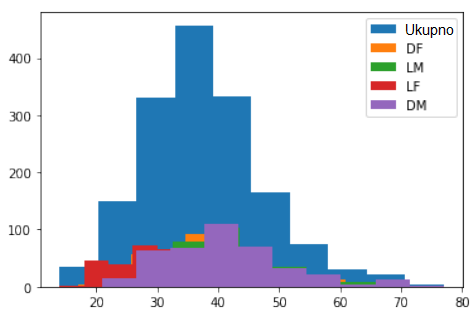
\includegraphics[width=0.4\linewidth]{hist.PNG}}
	\caption{\textbf{Histogram raspodele uzrasta u CelebSET-u. Medijana je 37, moda 36 a srednja vrednost 37.56. Najmlađa osoba ima 14 godina, dok najstarija ima 77. \textcolor{cc-purple}{Ljubičasta}, \textcolor{cc-orange}{narandžasta}, \textcolor{cc-green}{zelena} i \textcolor{cc-red}{crvena} odgovaraju raspodeli uzrasta redom crncima, belcima, crnkinjama i belkinjama.}}
	\label{fig:hist}
\end{figure}

\subsubsection{Konflikt 2: Intersekcionalna i grupna jednakost}
Koncept intersekcionalnosti, koji je prvi put upotrebila Krinšo \cite{G12}, je model koji objašnjava kako međusobno povezani sistemi privilegije i opresije utiču na iskustva pojedinaca koji poseduju karakteristike marginalizovanih grupa \cite{G13}. \\
\indent Krinšo navodi da treba napustiti ustaljene prakse i da odlukama treba pristupiti sa individualnog nivoa -- pojedinac se definiše kao presek mnogobrojnih kombinacija identiteta i sastoji se od nekoliko nivoa privilegije i opresije. Ovakva vrsta višečlane, odnosno višedimenzione analize ne uspeva da utvrdi kako sistemi privilegije i opresije utiču na iskustvo pojedinca koji poseduju kartakteristike marginalizovanih grupa \cite{G25}.\\
\indent \textbf{Ilustracija} Tokom razvoja CelebSET-a, posebna pažnju je posvećena ravnoteži prikupljenih oznaka o polu i binarnom polu upšte. Iako je takav dizajn proistekao iz oznaka prikupljenih iz pomenutih skupova podataka, podela na ovakve etničke grupe, kako je to izvršeno, nužno povlači izvesna ograničenja. Za razliku od \textit{Gender Shade} istraživanja \cite{G6}, gde su etničke grupe definisane u odnosu na boju kože, etnička pripadnost jeste visoko korelisana ali nedeterministički povezana sa rasnim podelama, što je u principu vrlo nejasan konstrukt, dajući pojedincima širok spektar fenotipskih karakteristika \cite{G3}. Slično, binarne oznake polova jesu u skladu sa načinom rada komercijalnih proizvoda, ali one koje su uklapaju u stereotipne opise polova nisu korišćene \cite{G29}. \\
\indent Figura \ref{fig:hist} pokazuje balansiranost polova i izražen disbalans uzrasta u CelebSET skupu podataka. Odsustvo nekih grupa je neizbežno -- deca ne smeju biti prisutna u ovakvom skupu podataka zbog pravnih načela. Prosečna starost tamnoputih žena je 37, belaca 39, belkinja 32, tamnoputih muškaraca 41. Budući da je mnogo veći broj belkinja od crnaca, nije očigledno da li do razlike u ovim grupama dolazi zbog rase ili pola. Moguće je, dakle, povećati performanse na polovima i etničkim grupama dok je istovremeno problem uzrast. Ovo je fenomen poznat kao \textit{džerimandering} \cite{G28}, gde se vrši kompromis jednakosti ortogonalnih ishoda.

\subsubsection{Konflikt 3: Transparentnost i prekomerna izloženost}
Da bi se umanjila mogućnost pogrešnog tumačenja rezultata verifikacije na konkretnim referentnim testovima, neophodno je pažljivo definisati ograničenja svakog skupa podataka i odgovarajuči domen upotrebe. Deljenjem detalja procesa kreiranja skupa podataka sa revizorima pomaže boljem razumevanju područja rada kao i konteksta u kom rezultate treba tumačiti. Objavljivanje tačnih ciljeva revizije proces verifikacije može učiniti značajno delotvornijim \cite{G39}. Međutim, to ima svoju cenu -- takav vid komunikacije može dovesti do kontraefekta poput preprilagođavanja reviziji. Pojedine kompanije su postale opreznije nakon revizije -- u septembru 2019. je IBM, kao predmet revizije \textit{Gender Shade} istraživanja, uklonio module za prepoznavanje lica u svom javno dostupnom API-u \cite{G26}. Slično, Kairos je svoje usluge načinio drastično skupljim nakon \textit{Actionable Auditing} istraživanja \cite{G27}. Takav trend, pored potpuno opravdanog povlačenja neispravnog softvera, onemogućava proveru takvog softvera -- čineći ga skupljim i otežavajući mu pristup, iako se njegova upotreba dozvoljava komercijalnim korisicnima. \\
\indent \textbf{Ilustracija} Ograničenja CelebSET-a kao i retrospektiva pristranosti su detaljno opisani u \cite{G20}. Tu je opisano koje su demografske grupe uključene u istraživanje i koji softver je pogodno testirati na CelebSET-u. Mogu se uočiti vrlo ograničene demografske grupe i mali opseg primene. IMDB-WIKI, kao skup iz kojeg je CelebSET izveden je javno dostupan \cite{G40}, te je celokupan proces kreiranja ovog skupa podataka transparentat i reproducibilan. To takođe znači i da su ciljevi revizije javni, što nužno znači da će ovaj skup podataka u jednom trenutku biti prevaziđen usled preprilagođavanja.

\section{Preispitivanje uloge algoritamske revizije}
Ispostavlja se da je algoritamsko revizionisanje poligon za evaluaciju etičkog pitanja. Revizija se mora obaviti vrlo pažljivo da ne bi došlo do problema koji se teže otkloniti, a revizori moraju ispuniti očekivanja kao da je reč o idealnom slučaju. \\
\indent Revizori, prema tome, provere vrše sa određenim nivoom tolerancije, uzimajući u obzir ograničenja sopstvenog načina provere i predstavljajući pojedinačne referentne rezultate kao osnovne delove daleko većeg i izražajnijeg frejmvorka. Cilj algoritamskog revizionisanja nije nužno ocena performansi, već oktrivanje zanemarenih komponenti. Imajući u vidu ograničenja ovakvog pristupa, revizija referentnim skupovima poput CelebSET-a je potrebna, ali ne i dovoljna. S tim u vezi, može se koristiti u cilju zastoja ili prekida razvoja, ali ne i kao preduslov za uvođenje moratorijuma. To znači da se dobar rezultat na CelebSET-u ne treba shvatiti kao krajnji cilj, već kao vrlo nizak prag koji se jednostavno mora ispoštovati.

\section{Zaključak}
Tokom kreiranja CelebSET-a, referentnog skupa podataka namenjenog proveri FPT proizvoda, uočeno je nekoliko etičkih prestupa, a uz to je i standardizovana algoritamska revizija vodećih proizvoda ovog tipa. Sumnja u etička načela revizije se uglavnom preklapa sa analogonom proizvoda koji se proverava, budući da neetički proces revizije može dovesti do pogrešne procene usaglašavanja FPT-a i uspostavljenih načela. Proces revizije kao i FPT podvrgnut reviziji moraju imati pažljivo razmotreno rešenje problema privatnosti. Takođe, moraju izbeći eksploataciju manjinskih grupa do koje može doći usled slepog praćenja poboljšanja rezultata. Ako se etičko pitanje revizije shvati ozbiljno, onda se istovetno mora pristupiti podacima kao i načinu provere.

\newpage
\begin{thebibliography}{9}
    \bibitem{G1} 
    Amazon. 2019. Amazon Rekognition FAQs.
    
    \bibitem{G2} 
    Ruha Benjamin. 2019. Race after technology: Abolitionist tools for the new jim code.
    John Wiley \& Sons.
    
    \bibitem{G3} 
    Sebastian Benthall and Bruce D. Haynes. 2019. Racial Categories in Machine
    Learning. In Proc. of the Conference on Fairness, Accountability, and Transparency (FAT). 10.
    
    \bibitem{G4}
    Sen. Roy Blunt. 2019. S.847 - Commercial Facial Recognition Privacy Act of 2019.
    
    \bibitem{G5}
    Joy Buolamwini. 2018. When the Robot Doesn’t See Dark Skin.
    
    \bibitem{G6}
    Joy Buolamwini and Timnit Gebru. 2018. Gender Shades: Intersectional Accuracy
    Disparities in Commercial Gender Classification. In Proc. of the Conference on
    Fairness, Accountability, and Transparency (FAT).
    
    \bibitem{G7}
    Matt Cagle and Nicole Ozer. 2018. Amazon Teams Up With Government to
    Deploy Dangerous New Facial Recognition Technology. (2018).
    
    \bibitem{G8}
    Clarifai. 2019. Custom Face Recognition.
    
    \bibitem{G9}
    Rep. Yvette D. Clarke. 2019. H.R.2231 - Algorithmic Accountability Act of 2019.
    
    \bibitem{G10}
    Rep. Yvette D. Clarke. 2019. H.R.4008 - No Biometric Barriers to Housing Act
    of 2019.
    
    \bibitem{G11}
    Lord Clement-Jones. 2019. Automated Facial Recognition Technology (Moratorium and Review) Bill [HL] 2019-20.
    
    \bibitem{G12}
    Kimberle Crenshaw. 1989. Demarginalizing the intersection of race and sex:
    A black feminist critique of antidiscrimination doctrine, feminist theory and
    antiracist politics. The University of Chicago Legal Forum (1989), 139.
    
    \bibitem{G13}
    Kimberle Crenshaw. 2017. Kimberle Crenshaw on Intersectionality, More than Two Decades Later.
    
    \bibitem{G14}
    Craig R Ehlen and Robert B Welker. 1996. Procedural fairness in the peer and quality review programs.
    Auditing 15, 1 (1996), 38.

    \bibitem{G15}
    Norman L Enger and Paul William Howerton. 1980.
    Computer Security: A Management Audit Approach. Amacom New York.
    
    \bibitem{G16}
    Face++. 2019. Face Attributes.

    \bibitem{G17}
    Sellywati Mohd Faizal, Mohd Rizal Palil, Ruhanita Maelah, and Rosiati Ramli.
    2017. Perception on justice, trust and tax compliance behavior in Malaysia.
    Kasetsart Journal of Social Sciences 38, 3 (2017), 226–232.

    \bibitem{G18}
    Sheera Frenkel. 2018. Microsoft Employees Question CEO Over Company’s Contract With ICE. (2018).
    
    \bibitem{G19}
    Timnit Gebru. 2019. Oxford Handbook on AI Ethics Book Chapter on Race and Gender.
    arXiv preprint arXiv:1908.06165 (2019).
    
    \bibitem{G20}
    Timnit Gebru, Jamie Morgenstern, Briana Vecchione, Jennifer Wortman Vaughan, Hanna Wallach, Hal Daume\'e III,
    and Kate Crawford. 2018. Datasheets for datasets. arXiv preprint arXiv:1803.09010 (2018).

    \bibitem{G21}
    Yandong Guo, Lei Zhang, Yuxiao Hu, Xiaodong He, and Jianfeng Gao. 2016.
    Ms-celeb-1m: Challenge of recognizing one million celebrities in the real world.
    Electronic imaging 2016, 11 (2016), 1–6.

    \bibitem{G22}
    Foad Hamidi, Morgan Klaus Scheuerman, and Stacy M Branham. 2018. Gender
    recognition or gender reductionism?: The social implications of embedded gender recognition systems.
    In Proc. of the ACM Conference on Human Factors in Computing Systems (CHI).

    \bibitem{G23}
    Amy Hawkins. 2018. Beijing's Big Brother Tech Needs African Faces.

    \bibitem{G24}
    Michael Hind, Sameep Mehta, Aleksandra Mojsilovic, Ravi Nair,
    Karthikeyan Natesan Ramamurthy, Alexandra Olteanu, and Kush R Varshney.
    2018. Increasing Trust in AI Services through Supplier’s Declarations of
    Conformity. arXiv preprint arXiv:1808.07261 (2018).

    \bibitem{G25}
    Anna Lauren Hoffmann. 2019. Where fairness fails: data, algorithms, and the
    limits of antidiscrimination discourse. Information, Communication \& Society 22,
    7 (2019), 900–915.

    \bibitem{G26}
    IBM. 2019. Release notes.

    \bibitem{G27}
    Kairos. 2019. Kairos Face Recognition Pricing Guide.

    \bibitem{G28}
    Michael Kearns, Seth Neel, Aaron Roth, and Zhiwei Steven Wu. 2018. Preventing
    Fairness Gerrymandering: Auditing and Learning for Subgroup Fairness. In Proc.
    of the International Conference on Machine Learning (ICML).

    \bibitem{G29}
    Os Keyes. 2018. The Misgendering Machines: Trans/HCI Implications of Automatic Gender Recognition.
    Proc. of the Human Computer Interact action 2, CSCW, Article 88 (Nov. 2018).

    \bibitem{G30}
    Steven Melendez. 2018. Despite a surge of tech activism, Clarifai plans to push
    further into government work. (2018).

    \bibitem{G31}
    Steven Melendez. 2018. Uber driver troubles raise concerns about
    transgender face recognition.

    \bibitem{G32}
    Michele Merler, Nalini Ratha, Rogerio S. Feris, and John R. Smith. 2019.
    Diversity in Faces. arXiv preprints, Article arXiv:1901.10436 (Jan. 2019),
    arXiv:1901.10436 pages.
    
    \bibitem{G33}
    Microsoft. 2019. What is the Azure Face API?
    
    \bibitem{G34}
    Margaret Mitchell, Simone Wu, Andrew Zaldivar, Parker Barnes, Lucy Vasserman,
    Ben Hutchinson, Elena Spitzer, Inioluwa Deborah Raji, and Timnit Gebru. 2018.
    Model Cards for Model Reporting. CoRR abs/1810.03993 (2018). arXiv preprint arXiv:1810.03993 (2018).
    
    \bibitem{G35}
    Paul Mozur. 2019. One Month, 500,000 Face Scans: How China Is Using A.I. to Profile a Minority. 
    
    \bibitem{G36}
    Kristina Murphy. 2003. Procedural justice and tax compliance. Australian Journal
    of Social Issues (Australian Council of Social Service) 38, 3 (2003).
    
    \bibitem{G37}
    Shruti Nagpal, Maneet Singh, Richa Singh, Mayank Vatsa, and Nalini Ratha.
    2019. Deep Learning for Face Recognition: Pride or Prejudiced? arXiv preprint
    arXiv:1904.01219 (2019).
    
    \bibitem{G38}
    Mei Ngan, Mei Ngan, and Patrick Grother. 2015. Face recognition vendor test
    (FRVT) performance of automated gender classification algorithms. Government
    Technical Report. US Department of Commerce, National Institute of Standards
    and Technology.
    
    \bibitem{G39}
    Inioluwa Deborah Raji and Joy Buolamwini. 2019. Actionable auditing: Investigating the impact of
    publicly naming biased performance results of commercial AI products. In Prof. of the Conference
    on Artificial Intelligence, Ethics, and Society.
    
    \bibitem{G40}
    Rasmus Rothe, Radu Timofte, and Luc Van Gool. 2016. Deep expectation of real
    and apparent age from a single image without facial landmarks. International
    Journal of Computer Vision (IJCV) (7 2016).
    
    \bibitem{G41}
    Silonie Sachdeva et al. 2009. Fitzpatrick skin typing: Applications in dermatology.
    Indian Journal of Dermatology, Venereology, and Leprology 75, 1 (2009), 93.
    
    \bibitem{G42}
    Morgan Klaus Scheuerman, Jacob M Paul, and Jedr Brubaker. 2019. How Computers See Gender:
    An Evaluation of Gender Classification in Commercial Facial Analysis and Image Labeling Services. (2019).

    \bibitem{G43}
    Jacob Snow. 2018. Amazon's Face Recognition Falsely Matched 28
    Members of Congress With Mugshots. 
    
    \bibitem{G44}
    Olivia Solon. 2019. Facial recognition’s ’dirty little secret’: Millions of online photos scraped without consent.
    
    \bibitem{G45}
    Nisha Srinivas, Karl Ricanek, Dana Michalski, David S Bolme, and Michael King.
    2019. Face Recognition Algorithm Bias: Performance Differences on Images of
    Children and Adults. In Proceedings of the IEEE Conference on Computer Vision and Pattern Recognition Workshops. 0-0.
\end{thebibliography}

\end{document}
